% Template for Cogsci submission with R Markdown

% Stuff changed from original Markdown PLOS Template
\documentclass[10pt, letterpaper]{article}

\usepackage{cogsci}
\usepackage{pslatex}
\usepackage{float}
\usepackage{caption}

% amsmath package, useful for mathematical formulas
\usepackage{amsmath}

% amssymb package, useful for mathematical symbols
\usepackage{amssymb}

% hyperref package, useful for hyperlinks
\usepackage{hyperref}

% graphicx package, useful for including eps and pdf graphics
% include graphics with the command \includegraphics
\usepackage{graphicx}

% Sweave(-like)
\usepackage{fancyvrb}
\DefineVerbatimEnvironment{Sinput}{Verbatim}{fontshape=sl}
\DefineVerbatimEnvironment{Soutput}{Verbatim}{}
\DefineVerbatimEnvironment{Scode}{Verbatim}{fontshape=sl}
\newenvironment{Schunk}{}{}
\DefineVerbatimEnvironment{Code}{Verbatim}{}
\DefineVerbatimEnvironment{CodeInput}{Verbatim}{fontshape=sl}
\DefineVerbatimEnvironment{CodeOutput}{Verbatim}{}
\newenvironment{CodeChunk}{}{}

% cite package, to clean up citations in the main text. Do not remove.
\usepackage{apacite}

% KM added 1/4/18 to allow control of blind submission
\cogscifinalcopy

\usepackage{color}

% Use doublespacing - comment out for single spacing
%\usepackage{setspace}
%\doublespacing


% % Text layout
% \topmargin 0.0cm
% \oddsidemargin 0.5cm
% \evensidemargin 0.5cm
% \textwidth 16cm
% \textheight 21cm

\title{A synthesis of early cognitive and language development using
(meta-)meta-analysis}

\usepackage{booktabs}
\usepackage{longtable}
\usepackage{array}
\usepackage{multirow}
\usepackage{wrapfig}
\usepackage{float}
\usepackage{colortbl}
\usepackage{pdflscape}
\usepackage{tabu}
\usepackage{threeparttable}
\usepackage{threeparttablex}
\usepackage[normalem]{ulem}
\usepackage{makecell}
\usepackage{xcolor}

\author{Anjie Cao$^1$  (anjiecao@stanford.edu)
 and \bf{Michael C. Frank$^1$ (mcfrank@stanford.edu)} \\
$^1$Department of Psychology, Stanford University, }

\newlength{\cslhangindent}
\setlength{\cslhangindent}{1.5em}
\newenvironment{CSLReferences}%
  {}%
  {\par}

\begin{document}

\maketitle

\begin{abstract}
HAHA

\textbf{Keywords:}
pikachu; mimikyu; ditto; jigglypufff
\end{abstract}

\hypertarget{introduction}{%
\section{Introduction}\label{introduction}}

In the first three years of life, children undergo a plethora of
developmental changes, transitioning from newborn infants who possess a
limited understanding of language and categories to toddlers who are
able to master a wide range of linguistic and cognitive skills. Despite
a wealth of research examining cognitive development, constructing a
comprehensive theory of cognitive development remains a formidable
challenge. Research in this area generally falls under two categories:
observational research and experimental research. Observational studies
using instruments like the Bayley Scales can provide a holistic picture
of an individual child's development {[}e.g.@bayley2006bayley{]}, but it
is a challenge to move from global developmental milestones to
underlying mechanisms. In contrast, experimental research allows causal
tractions on potential mechanisms, but experiments typically focus on
one single construct and does not reveal the connections between
different processes and mechanisms. In this paper, we aim to provide a
quantitative synthesis of experimental work across multiple areas of
developmental psychology, providing insights into the interrelatedness
between psychological constructs. We achieve this goal by consolidating
and integrating 23 meta-analyses of cognitive and language development
compiled on MetaLab, a community-augmented meta-analysis platform.

Statistical meta-analysis, the technique of aggregating effect sizes
across a systematic sample of experiments, has some unique advantages as
a source of data about developmental processes in early childhood. First
and foremost, it allows researchers to explore questions that are
difficult to address with individual studies. One such example is the
functional form of developmental curves, or how different psychological
processes change over time. Many developmental studies use linear
regression models with age as a predictor, but this assumption of
linearity may not capture the complexities of developmental processes,
especially as they interact with developmental changes in measurement.
For example, some cognitive abilities -- such as relational reasoning --
might follow an inverted-U shape (Carstensen et al., 2019; Walker,
Bridgers, \& Gopnik, 2016), while others -- like early vocabulary size
-- show an exponential increase (Frank, Braginsky, Yurovsky, \&
Marchman, 2021). These non-linear trends can be challenging to identify
and interpret with limited data from individual studies, but
meta-analytic methods can provide a large amount of data across a broad
age range, enabling researchers to evaluate and compare different
functional forms of developmental trajectories.

Meta-analysis can also shed light on the relationships between methods
and theories. Research methods and theories are fundamentally
intertwined, and this is especially true for developmental psychology
{[}@\hspace{0pt}\hspace{0pt}dale2022fundamental{]}. Developmental
theories are often based on interpretations of experimental results,
which are produced by methods that even small changes to the parameters
would substantially change the outcomes. One example is the influence of
familiarization time. It has been proposed that the amount of exposure
infants have prior to the test events can influence infants' direction
of preference (i.e.~novelty preference or familiarity preference)
(Hunter \& Ames, 1988). Although the empirical evidence for this theory
is mixed, this ambiguity has significant downstream consequences on our
understanding of infants' cognitive capabilities (Bergmann \& Cristia,
2016). Debates about infants' arithmetic competencies or their
evaluations of social agents are often centered around the direction of
preferences (Infants arithmetic competencies: Clearfield \& Westfahl,
2006; Wakeley, Rivera, \& Langer, 2000; Wynn, 1993; Evaluation of social
agents: Hamlin, Wynn, \& Bloom, 2007; Salvadori et al., 2015). Due to
the time and resources required for developmental studies, it is often
difficult to directly evaluate the impact of subtle changes in
parameters. Therefore, meta-analytic methods provide a unique
opportunity to investigate the effects of methodological factors on
research findings.

Last but not least, meta-analytic methods make it possible to compare
and connect research findings across research areas. The use of effect
size as the fundamental unit of analysis allows for comparisons across
different domains and research areas. These comparisons can provide
insight into how different processes facilitate learning at different
stages of development and can aid in the development of data-driven
cognitive development theories (Cao \& Lewis, 2022; Lewis et al., 2016).
However, a synthesis across multiple domains requires a database of
multiple meta-analyses. Towards that aim, MetaLab was established to
provide an open database of meta-analyses (Bergmann et al., 2018).
Developmental researchers are invited to deposit their meta-analysis
dataset into MetaLab, and they are encouraged to use the datasets for
custom analyses. As of November 2022, Metalab contains X effect sizes
from 30 different meta-analyses. This resource allows the beginnings of
a quantitative synthesis across different research areas in
developmental psychology.

In particular, we address three separate questions. First, we would like
to investigate the shape of developmental curves across domains. The
form of growth curves has been of interest in a lot of areas of
developmental research (e.g., exponential growths in vocabulary:
McMurray, 2007; asymptotic decreases in reaction time: Kail, 1991) These
nuanced descriptions of developmental trajectories allow for a more
precise understanding of the underlying mechanisms driving these
changes. We aim to provide these quantitative descriptions for more
research areas. Second, we hope to understand how research methods
moderate the strengths of the findings. Increasingly, developmental
research methods are scrutinized for their mechanisms and scientific
rigors (Paulus, 2022; Stahl \& Kibbe, 2022). With MetaLab, the fields
are ripe for a more systematic understanding of how different design
choices in experiments could influence the results. Finally, we would
like to offer a birds-eye view of the field by integrating the growth
curves across multiple domains. This view would provide an empirical
foundation for creating a synthesized theory of cognitive development.

The plan for this paper is as follows. We first describe the datasets
included in the current synthesis, including our selection criteria and
the descriptive statistics associated with our final dataset. We then
turn to model comparison, comparing the fits of age models under
different functional forms. Next, we present methodological moderators
analysis. Four methodological moderators are selected due to their
theoretical relevances: behavioral measure type, exposure phase type,
stimuli naturalness, and major author effect. Finally, we present a
synthesis of the developmental curves across all of the domains
considered. We end the paper by discussing the implications and
limitations of our current work.

\hypertarget{methods}{%
\section{Methods}\label{methods}}

\hypertarget{datasets}{%
\subsection{Datasets}\label{datasets}}

Datasets were retrieved from \texttt{metalabr}, the R package built from
Metalab. As of November 2022, the package includes 30 individual
meta-analysis datasets covering different research domains in language
learning and cognitive development. We removed 5 datasets from the final
analysis, including 2 with data quality issues (Word segmentation neuro;
Phonotactic learning), 3 due to being observational studies or including
studies with quasi-experimental design (Pointing and vocabulary
concurrent; Pointing and vocabulary, longitudinal; Video deficit)). We
modified 2 datasets to reflect a more accurate representation of the
literature and combined two pairs of datasets because they measure
theoretically identical constructs. To minimize the heterogeneity in our
datasets, we also excluded effect sizes calculated from participants
with clinical diagnoses.

The final dataset contained 23 meta-analyses. Table 1 provides a summary
of the, along with the number of effect sizes and participants included
in each dataset.

The final dataset and analysis scripts are available at X.

\hypertarget{analytic-methods}{%
\subsection{Analytic Methods}\label{analytic-methods}}

All analyses were conducted in R using the \texttt{metafor} package
(Viechtbauer, 2010). We specified multi-level random effect models with
random effect structures that included grouping by paper and by
participant group. We removed the clustering if grouping information was
missing from the dataset. All moderators were included as fixed effects.
Unless otherwise specified, all model comparisons were based on the
corrected Akaike Information Criterion (AICc).

\hypertarget{results}{%
\section{Results}\label{results}}

\hypertarget{functional-form-of-developmental-curves}{%
\subsection{Functional form of developmental
curves}\label{functional-form-of-developmental-curves}}

\begin{table*}
\begin{tabular}{l|r|r|r|r|r|r|r}

\hline
\textbf{Dataset} & N ES & N Participants & ES & Linear & Log & Quadratic & Constant\\
\hline
Label advantage in concept learning & 100 & 1644 & 0.36 & 169.48 & \textbf{168.53} & 170.16 & 170.89\\
Vowel discrimination (native) & 143 & 2418 & 0.59 & 256.49 & 256.13 & 256.78 & \textbf{255.15}\\
Vowel discrimination (non-native) & 49 & 600 & 0.65 & 73.25 & 73.36 & 73.15 & \textbf{71.69}\\
Statistical word segmentation & 103 & 804 & -0.08 & 128.84 & 129.01 & 128.62 & \textbf{127.50}\\
Online word recognition & 14 & 330 & 1.37 & \textbf{46.50} & 46.73 & 46.65 & 48.72\\
Mutual exclusivity & 131 & 2222 & 1.27 & 421.60 & \textbf{415.85} & 432.76 & 453.07\\
Sound symbolism & 44 & 425 & 0.16 & 58.20 & \textbf{58.16} & 58.83 & 61.04\\
Categorization bias & 80 & 382 & 0.25 & 300.29 & \textbf{299.99} & 300.37 & 300.90\\
Familiar word recognition & 34 & 586 & 0.54 & 27.46 & 28.32 & \textbf{27.18} & 28.86\\
Abstract rule learning & 95 & 1123 & 0.22 & 140.80 & 141.34 & \textbf{140.47} & 140.91\\
Switch task & 143 & 2764 & -0.16 & 204.79 & 204.81 & 204.73 & \textbf{203.67}\\
Mispronunciation sensitivity & 249 & 2122 & 0.45 & 620.05 & 628.16 & \textbf{613.67} & 644.40\\
Prosocial agents & 61 & 1244 & 0.40 & 82.16 & 81.95 & 82.23 & \textbf{80.08}\\
Simple arithmetic competences & 14 & 369 & 0.25 & 22.91 & 23.01 & 22.81 & \textbf{16.26}\\
Symbolic play & 196 & 7148 & 0.63 & 234.15 & 234.11 & 234.13 & \textbf{233.57}\\
Natural speech preference & 55 & 786 & 0.44 & 111.40 & 112.01 & \textbf{110.97} & 111.83\\
Cross-situational word learning & 48 & 2241 & 0.67 & 79.81 & 81.62 & \textbf{79.70} & 83.71\\
Language discrimination and preference & 153 & 2060 & -0.13 & 264.70 & 265.59 & \textbf{262.65} & 264.95\\
Syntactic bootstrapping & 60 & 832 & 0.24 & 107.28 & \textbf{106.99} & 107.57 & 107.47\\
Statistical sound category learning (habituation) & 11 & 350 & 0.56 & 33.47 & 34.54 & 32.94 & \textbf{30.46}\\
Gaze following (combined) & 81 & 1407 & 0.81 & 151.53 & 159.88 & \textbf{149.47} & 193.20\\
Word Segmentation (combined) & 315 & 2910 & 0.20 & 328.83 & 328.60 & 329.16 & \textbf{327.55}\\
Infant directed speech preference & 83 & 985 & 0.47 & 70.17 & 70.87 & 70.06 & \textbf{69.13}\\
\hline
\end{tabular}
\caption{\label{demo-table}Your caption.}
\end{table*}

Our first research question was about the functional form of the
developmental trajectories we observed. We considered four specific
forms: linear, logarithmic, quadratic, and constant, each considered as
an age-related fixed effect. We evaluated the models based on the
corrected AICc (Table 1). 10 out of the 23 datasets had the constant
model as the best-fitting model. 7 and 5` datasets' best-fitting models
are the Quadratic model and logarithmic model, respectively. Finally,
among all datasets considered, Online Word Recognition was the only
domain in which the linear age model provides the best fit. Model
evaluation based on Bayesian Information Criterion (BIC) yielded similar
results with little discrepancy.

\hypertarget{methodological-moderators}{%
\subsection{Methodological Moderators}\label{methodological-moderators}}

In this section, we considered methodological moderators shared by
multiple datasets. Given the limited number of studies conducted with
neuroimaging methods, we focused our analyses on studies conducted with
behavioral methods. Therefore, we excluded studies that were conducted
with either fNIRS or EEG. Moreover, to minimize age-related
heterogeneity, we only included studies with participants' mean age
below 36 months. All analyses were conducted on the subset of research
domains with multiple levels for the moderator of interests.

Figure 1 provides a summary of the estimates for moderators.

\hypertarget{behavioral-measures}{%
\subsubsection{Behavioral Measures}\label{behavioral-measures}}

Meta-analyses have very heterogeneous moderators coded, but many
included coding of which behavioral response measure was used in the
original study: looking-based behaviors (e.g., looking time or other
eye-tracking measures), sucking (as in the high amplitude sucking
procedure), and manual behaviors (e.g., pointing, exploration). We thus
added behavioral measure as an additional fixed effect to the age model
with the best-fitting functional form from the previous analysis.

In general, nearly all effects were weakly positive such that sucking
and manual response modes yielded slightly larger effect sizes, though
these effects were not always significant. Behavioral measure was a
significant predictor of effect sizes in only two domains, Vowel
Discrimination (Native) and Sound Symbolism. In Vowel Discrimination
(native), studies with Manual or Sucking behavioral measure has larger
effect sizes than studies using looking as the behavioral measure
(Manual: \(\beta\) = 0.58 {[}0.33, 0.82{]}, \emph{z} = 4.6, \emph{p}
\textless{} 0.01 ; Sucking: \(\beta\) = 0.96 {[}0.53, 1.4{]}, \emph{z} =
4.34, \emph{p} \textless{} 0.01). Similarly, in Sound Symbolism, studies
with manual behavioral measures also yield larger effect sizes than
looking studies (\(\beta\) = 0.61 {[}0.24, 0.97{]}, \emph{z} = 3.29,
\emph{p} \textless{} 0.01).

We also explored whether there would be an interaction between the
research methods and the age of participants. There was limited evidence
for such interaction. The inclusion of interaction terms only improved
the AICc in 3 domains (Label advantage in concept learning; Language
discrimination and preference; Mutual exclusivity). Of all the
interaction models, only the Language discrimination and preference
showed a significant positive interaction effect between the manual
behavioral measure and age (\(\beta\) = 0.01 {[}0, 0.02{]}, \emph{z} =
2.19, \emph{p} = 0.03).

\hypertarget{exposure-phase}{%
\subsubsection{Exposure Phase}\label{exposure-phase}}

Exposure phase refers to the type of exposure infants have during the
experiments prior to the test events. There are typically four types of
exposure phase: 1) an infant would be conditioned to show an orienting
behavior (conditioning); 2) an infant would be exposed to a stimulus for
a constant amount of time (familiarization); 3) an infant would be shown
some stimulus repeatedly until the magnitude of response drops below a
threshold (habituation); 4) no exposure to the stimulus at all; the
infant would be tested immediately (test-only). We coded these four
types of exposure phases as four levels in the moderator exposure phase.

Exposure phase is a significant predictor of effect sizes in four
domains. In Language Discrimination and Preference, habituation studies
yield smaller effect sizes than conditioning studies (\(\beta\) = -0.3
{[}-0.55, -0.04{]}, \emph{z} = -2.28, \emph{p} = 0.02). A similar trend
is found in Vowel discrimination (native), where both habituation
studies and familiarization studies have smaller effect sizes than
conditioning studies (Habituation: \(\beta\) = -0.71 {[}-1.11, -0.31{]},
\emph{z} = -3.48, \emph{p} \textless{} 0.01; Familiarization: \(\beta\)
= -0.43 {[}-0.87, 0.01{]}, \emph{z} = -1.94, \emph{p} = 0.05).

Interestingly, the results of the comparison between familiarization
studies and conditioning studies are mixed. In the Vowel discrimination
(non-native) dataset, both familiarization and test-only studies produce
smaller effect sizes than the conditioning studies (Familiarization:
\(\beta\) = -1.4 {[}-2.35, -0.46{]}, \emph{z} = -2.93, \emph{p}
\textless{} 0.01; Test-only: \(\beta\) = -1.26 {[}-2.42, -0.1{]},
\emph{z} = -2.13, \emph{p} = 0.03). However, the opposite trend is found
in Natural Speech Preference, with familiarization studies producing
larger effect sizes than the conditioning studies (\(\beta\) = 1.65
{[}0.33, 2.97{]}, \emph{z} = 2.44, \emph{p} = 0.01).

\hypertarget{stimuli-naturalness}{%
\subsubsection{Stimuli Naturalness}\label{stimuli-naturalness}}

Next, we considered the effect of stimuli type. We focused on one key
dimension: naturalness. For primarily visual stimuli, we considered
``naturalness'' to mean stimuli that use real-world objects
(e.g.~puppets, blocks). We compared these natural stimuli with
representation-type stimuli, such as pictures, videos, or drawings. In
primarily auditory stimuli, we compared natural speech with synthesized
stimuli.

We found that naturalness is a significant predictor for Label advantage
in concept learning, with natural stimuli yielding larger effect sizes
than representation-type stimuli (\(\beta\) = 0.23 {[}0.01, 0.45{]},
\emph{z} = 2.06, \emph{p} = 0.04). Similarly, in both Statistical word
segmentation and Abstract rule learning, we found a natural speech
advantage (Statistical word segmentation: \(\beta\) = 0.47 {[}0.23,
0.72{]}, \emph{z} = 3.8, \emph{p} \textless{} 0.01; Abstract rule
learning: \(\beta\) = 0.27 {[}0.05, 0.5{]}, \emph{z} = 2.35, \emph{p} =
0.02).

\begin{CodeChunk}
\begin{figure*}[h]

{\centering 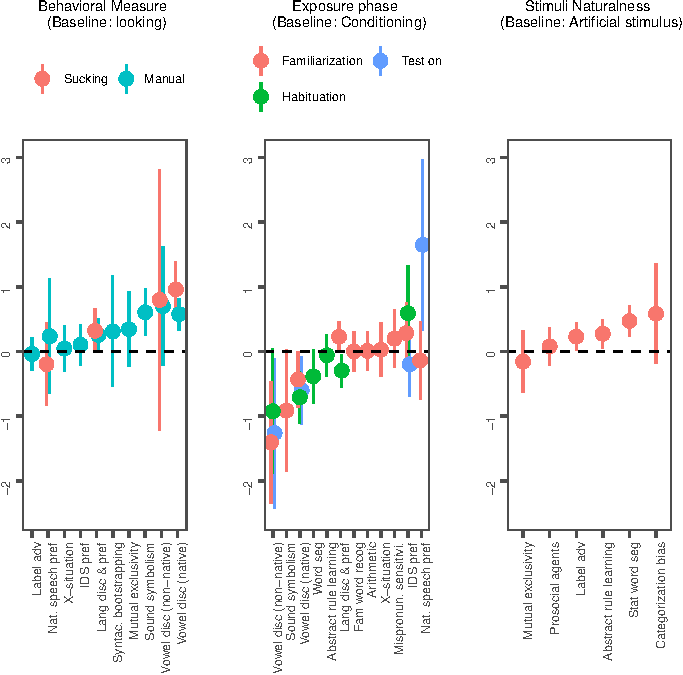
\includegraphics{figs/2-col-image-1} 

}

\caption[This image spans both columns]{This image spans both columns. And the caption text is limited to 0.8 of the width of the document.}\label{fig:2-col-image}
\end{figure*}
\end{CodeChunk}

\hypertarget{major-author}{%
\subsubsection{Major author}\label{major-author}}

Margoni \& Surian (2018) found evidence for an author-based bias in
Prosocial Agents, where results produced by certain authors were
consistently larger than others. We evaluated how prevalent this
phenomenon was in the literature by coding a ``major author'' moderator.
Authors are considered to be a ``major author'' if they are listed as
authors in more than 15\% of the papers in the literature.

We found evidence for a major author effect in 7 datasets, where studies
produced by the major author were larger than the rest of the papers. In
3 datasets, however, we also found the opposite patterns, where certain
authors produced on average smaller effect sizes than the rest of the
literature.

\begin{CodeChunk}
\begin{figure}[H]

{\centering 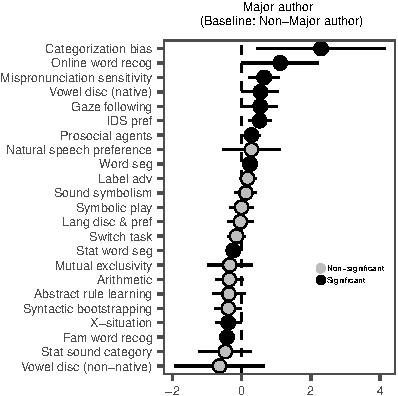
\includegraphics{figs/image-1} 

}

\caption[One column image]{One column image.}\label{fig:image}
\end{figure}
\end{CodeChunk}

\hypertarget{synthesis}{%
\subsection{Synthesis}\label{synthesis}}

Finally, we synthesized all 23 datasets by grouping them based on the
type of theoretical constructs they represented: Cognitive,
Communication, Sounds, and Words. We integrated the predictions from the
best-fitting age-based models in Figure 2, showing predictions across
the range of measured phenomena. We found a striking range of functional
forms in the developmental trajectories across all types of theoretical
constructs. In particular, the magnitudes of some phenomena -- online
word recognition, gaze following, and mutual exclusivity, for example --
increased substantially over development. In contrast, others -- sound
symbolism, categorization bias, and others -- stayed constant at a
measurable level without showing developmental increases. We considered
several explanations for these differences: one is that these
meta-analyses might correspond to relatively more experience-independent
biases. On the other hand, we cannot rule out cross-experiment
confounding wherein experimenters test progressively harder stimuli with
development, thus counteracting any developmental gains that might
otherwise be measured.

\hypertarget{discussion}{%
\section{Discussion}\label{discussion}}

How can we quantitatively describe developmental growth at scale?
Meta-analysis is one promising method. In this paper, we presented a
bird-eye view of developmental psychology by synthesizing 23
meta-analyses available on MetaLab. We found great diversity in the
shapes of the best-fitting models for each domain -- while some
phenomena showed larger and larger effects with development, quite a
number of others stayed constant, suggesting a distinction between small
but measurable in-lab effects and behaviors that can easily be observed
in individual children (effect sizes \textgreater{} 2). We also
considered the moderating effects of different methodological factors,
including the type of behavioral measure, the type of exposure phase,
stimuli naturalness, and whether the work is done by a ``major author''.
These factors moderate effect sizes from different domains in
heterogeneous ways, though we did find evidence for naturalistic stimuli
leading to larger effects in a number of studies.

\begin{CodeChunk}
\begin{figure*}[h]

{\centering 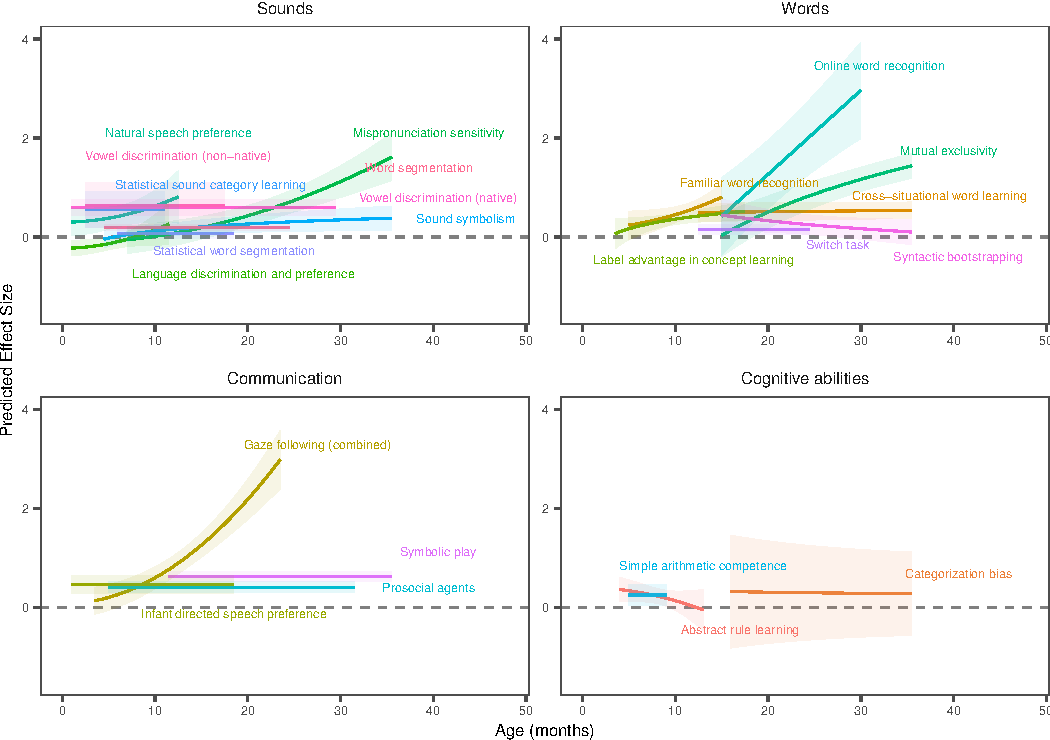
\includegraphics{figs/2-col-imageb-1} 

}

\caption[This image spans both columns]{This image spans both columns. And the caption text is limited to 0.8 of the width of the document.}\label{fig:2-col-imageb}
\end{figure*}
\end{CodeChunk}

This current synthesis highlights the variation in developmental
trajectories, challenging the traditional ``milestone'' view of
cognitive development. Under the milestone view, infants would acquire
different cognitive and linguistic skills as they grow (Meylan \&
Bergelson, 2022; Wilks, Gerber, \& Erdie-Lalena, 2010). Our findings
suggest that this view is missing two important details. First, at any
given age, psychological constructs could have a wide range of effect
sizes. For example, at 15 months of age, the predicted effect sizes for
communication skills range from X (DOMAIN NAME) to X (DOMAIN NAME). The
differences between the strengths of the effect may reflect the
differences in how these skills contribute to communication, with some
playing a more significant role than others. In addition, the
development of these skills could follow significantly different
trajectories, with some increasing exponentially with age and others
staying constant throughout early childhood. The heterogeneity of the
developmental process calls for developing a more nuanced and integrated
developmental theory.

The heterogeneity can also partly be attributed to the wide variety of
research methods. In the current analysis, we focused on in-lab
experimental work, and thus the effect sizes may as well reflect how
well the research methods capture the phenomenon of interest. Indeed, we
have shown that subtle experimental procedure changes (e.g.~exposure
phase) could significantly alter the effect sizes. Moreover, methods'
impact varies across domains, with some domains being more susceptible
to methodological factors than others. Therefore, the developmental
trajectories that we document could be influenced by researchers
adapting their methods to participants of different ages. In fact, we
have found that the inclusion of methodological moderators could change
the functional form of the best-fitting models. For example, in Infant
Directed Speech preference, the winning functional form for an age-only
model is constant (STATS? ). However, when the Exposure Phase moderator
is included, the best-fitting model includes age as a linear term
(STATS? ). Our findings call attention to the importance of
understanding methods' nuances: rather than treating methods as a
perfect mirror perfectly reflecting the phenomenon, they should be
regarded as an imperfect lens that could distort our perception of the
phenomenon.

Of course, the same can be said about meta-analysis. Meta-analysis is
not a perfect tool, and can often produce effect sizes significantly
larger than a comparable large-scale replication (Kvarven, Strømland, \&
Johannesson, 2020). Part of the discrepancy can be attributed to the
heterogeneity of research methods that are often minimized in a
large-scale replication (Lewis, Mathur, VanderWeele, \& Frank, 2020).
While we have included methodological moderators in our analysis, it is
highly likely that the coded moderators did not fully reflect the
subtlety of research methods. However, the ``Major author'' effect found
in many research domains could provide a window into understanding the
workings of the research method. In the future, we could compare and
contrast the methods used by ``major authors'' and those by others.
Doing so would allow us to pinpoint the differences and understand which
aspects of the methods really matter, and which do not.

Our ultimate goal is to offer a data-driven synthetic theory of
cognitive development. Here we have made our first step toward that goal
by offering a synthesis of meta-analyses across 23 different research
domains. Moving forward, we aim to expand and refine our synthesis by
including more research areas, correcting potential publication biases,
and accounting for more detailed methodological factors. We would also
like to make more connections between our meta-analysis-based work and
the many ongoing analyses based on large-scale multi-site replication
projects (e.g.~ManyBabies: Frank et al., 2017). Ultimately, we hope our
analysis could provide a solid empirical foundation to help us to better
understand the complex and diverse processes involved in cognitive
development.

\hypertarget{references}{%
\section{References}\label{references}}

\setlength{\parindent}{-0.1in} 
\setlength{\leftskip}{0.125in}

\noindent

\hypertarget{refs}{}
\begin{CSLReferences}{1}{0}
\leavevmode\vadjust pre{\hypertarget{ref-bergmann2016development}{}}%
Bergmann, C., \& Cristia, A. (2016). Development of infants'
segmentation of words from native speech: A meta-analytic approach.
\emph{Developmental Science}, \emph{19}(6), 901--917.

\leavevmode\vadjust pre{\hypertarget{ref-bergmann2018promoting}{}}%
Bergmann, C., Tsuji, S., Piccinini, P. E., Lewis, M. L., Braginsky, M.,
Frank, M. C., \& Cristia, A. (2018). Promoting replicability in
developmental research through meta-analyses: Insights from language
acquisition research. \emph{Child Development}, \emph{89}(6),
1996--2009.

\leavevmode\vadjust pre{\hypertarget{ref-cao2022quantifying}{}}%
Cao, A., \& Lewis, M. (2022). Quantifying the syntactic bootstrapping
effect in verb learning: A meta-analytic synthesis. \emph{Developmental
Science}, \emph{25}(2), e13176.

\leavevmode\vadjust pre{\hypertarget{ref-carstensen2019context}{}}%
Carstensen, A., Zhang, J., Heyman, G. D., Fu, G., Lee, K., \& Walker, C.
M. (2019). Context shapes early diversity in abstract thought.
\emph{Proceedings of the National Academy of Sciences}, \emph{116}(28),
13891--13896.

\leavevmode\vadjust pre{\hypertarget{ref-clearfield2006familiarization}{}}%
Clearfield, M. W., \& Westfahl, S. M.-C. (2006). Familiarization in
infants' perception of addition problems. \emph{Journal of Cognition and
Development}, \emph{7}(1), 27--43.

\leavevmode\vadjust pre{\hypertarget{ref-frank2017collaborative}{}}%
Frank, M. C., Bergelson, E., Bergmann, C., Cristia, A., Floccia, C.,
Gervain, J., et al.others. (2017). A collaborative approach to infant
research: Promoting reproducibility, best practices, and
theory-building. \emph{Infancy}, \emph{22}(4), 421--435.

\leavevmode\vadjust pre{\hypertarget{ref-frank2021variability}{}}%
Frank, M. C., Braginsky, M., Yurovsky, D., \& Marchman, V. A. (2021).
\emph{Variability and consistency in early language learning: The
wordbank project}. MIT Press.

\leavevmode\vadjust pre{\hypertarget{ref-hamlin2007social}{}}%
Hamlin, J. K., Wynn, K., \& Bloom, P. (2007). Social evaluation by
preverbal infants. \emph{Nature}, \emph{450}(7169), 557--559.

\leavevmode\vadjust pre{\hypertarget{ref-hunter1988multifactor}{}}%
Hunter, M. A., \& Ames, E. W. (1988). A multifactor model of infant
preferences for novel and familiar stimuli. \emph{Advances in Infancy
Research}.

\leavevmode\vadjust pre{\hypertarget{ref-kail1991developmental}{}}%
Kail, R. (1991). Developmental change in speed of processing during
childhood and adolescence. \emph{Psychological Bulletin}, \emph{109}(3),
490.

\leavevmode\vadjust pre{\hypertarget{ref-kvarven2020comparing}{}}%
Kvarven, A., Strømland, E., \& Johannesson, M. (2020). Comparing
meta-analyses and preregistered multiple-laboratory replication
projects. \emph{Nature Human Behaviour}, \emph{4}(4), 423--434.

\leavevmode\vadjust pre{\hypertarget{ref-lewis2016quantitative}{}}%
Lewis, M., Braginsky, M., Tsuji, S., Bergmann, C., Piccinini, P. E.,
Cristia, A., et al. (2016). A quantitative synthesis of early language
acquisition using meta-analysis.

\leavevmode\vadjust pre{\hypertarget{ref-lewis2020puzzling}{}}%
Lewis, M., Mathur, M., VanderWeele, T., \& Frank, M. C. (2020). The
puzzling relationship between multi-lab replications and meta-analyses
of the rest of the literature.

\leavevmode\vadjust pre{\hypertarget{ref-margoni2018infants}{}}%
Margoni, F., \& Surian, L. (2018). Infants' evaluation of prosocial and
antisocial agents: A meta-analysis. \emph{Developmental Psychology},
\emph{54}(8), 1445.

\leavevmode\vadjust pre{\hypertarget{ref-mcmurray2007defusing}{}}%
McMurray, B. (2007). Defusing the childhood vocabulary explosion.
\emph{Science}, \emph{317}(5838), 631--631.

\leavevmode\vadjust pre{\hypertarget{ref-meylan2022learning}{}}%
Meylan, S. C., \& Bergelson, E. (2022). Learning through processing:
Toward an integrated approach to early word learning. \emph{Annual
Review of Linguistics}, \emph{8}, 77--99.

\leavevmode\vadjust pre{\hypertarget{ref-paulus2022should}{}}%
Paulus, M. (2022). Should infant psychology rely on the
violation-of-expectation method? Not anymore. \emph{Infant and Child
Development}, \emph{31}(1), e2306.

\leavevmode\vadjust pre{\hypertarget{ref-salvadori2015probing}{}}%
Salvadori, E., Blazsekova, T., Volein, A., Karap, Z., Tatone, D.,
Mascaro, O., \& Csibra, G. (2015). Probing the strength of infants'
preference for helpers over hinderers: Two replication attempts of
hamlin and wynn (2011). \emph{PloS One}, \emph{10}(11), e0140570.

\leavevmode\vadjust pre{\hypertarget{ref-stahl2022great}{}}%
Stahl, A. E., \& Kibbe, M. M. (2022). Great expectations: The construct
validity of the violation-of-expectation method for studying infant
cognition. \emph{Infant and Child Development}, \emph{31}(6), e2359.

\leavevmode\vadjust pre{\hypertarget{ref-viechtbauer2010conducting}{}}%
Viechtbauer, W. (2010). Conducting meta-analyses in r with the metafor
package. \emph{Journal of Statistical Software}, \emph{36}(3), 1--48.

\leavevmode\vadjust pre{\hypertarget{ref-wakeley2000can}{}}%
Wakeley, A., Rivera, S., \& Langer, J. (2000). Can young infants add and
subtract? \emph{Child Development}, \emph{71}(6), 1525--1534.

\leavevmode\vadjust pre{\hypertarget{ref-walker2016early}{}}%
Walker, C. M., Bridgers, S., \& Gopnik, A. (2016). The early emergence
and puzzling decline of relational reasoning: Effects of knowledge and
search on inferring abstract concepts. \emph{Cognition}, \emph{156},
30--40.

\leavevmode\vadjust pre{\hypertarget{ref-wilks2010developmental}{}}%
Wilks, T., Gerber, R. J., \& Erdie-Lalena, C. (2010). Developmental
milestones: Cognitive development. \emph{Pediatrics in Review},
\emph{31}(9), 364--367.

\leavevmode\vadjust pre{\hypertarget{ref-wynn1993erratum}{}}%
Wynn, K. (1993). Erratum: Addition and subtraction by human infants.
\emph{Nature}, \emph{361}(6410), 374--374.

\end{CSLReferences}

\bibliographystyle{apacite}


\end{document}
